% You should title the file with a .tex extension (hw1.tex, for example)
\documentclass[11pt]{article}

\usepackage{amsmath}
\usepackage{mathtools}
\usepackage{amssymb}
\usepackage{fancyhdr}
\usepackage{tikz-qtree}
\usepackage{tikz-qtree-compat}
\usepackage[normalem]{ulem}
\usepackage{tikz}
\usepackage{graphicx}
\DeclareMathOperator*{\argmin}{argmin}
\DeclareMathOperator*{\argmax}{argmax}

\oddsidemargin0cm
\topmargin-2cm     %I recommend adding these three lines to increase the 
\textwidth16.5cm   %amount of usable space on the page (and save trees)
\textheight23.5cm  

\newcommand{\question}[2] {\vspace{.25in} \hrule\vspace{0.5em}
\noindent{\bf #1: #2} \vspace{0.5em}
\hrule \vspace{.10in}}
\renewcommand{\part}[1] {\vspace{.10in} {\bf (#1)}}

\newcommand{\myname}{Sean Bittner}
\newcommand{\myandrew}{srb2201@columbia.edu}
\newcommand{\myhwnum}{12}

\setlength{\parindent}{0pt}
\setlength{\parskip}{5pt plus 1pt}
 
\DeclarePairedDelimiter\abs{\lvert}{\rvert}%
 
\pagestyle{fancyplain}
\rhead{\fancyplain{}{\myname\\ \myandrew}}

\begin{document}

\medskip                        % Skip a "medium" amount of space
                                % (latex determines what medium is)
                                % Also try: \bigskip, \littleskip

\thispagestyle{plain}
\begin{center}                  % Center the following lines
{\Large Damped harmonic oscillator DSN hyperparameter search} \\
Aug 28, 2018 \\
\end{center}
\question{1}{Damped harmonic oscillator}
The classical damped harmonic oscillator is a good system to show proof of principle with DSNs.  A DHO models a system often described as a swinging mass acted on by forces of gravity, a spring, and friction.  The dynamics are described by the simple equation:
\[m \frac{d^2 x}{dt^2} = kx + c \frac{dx}{dt} \]
with parameters corresponding to mass $m$, fricition coefficient $c$ and spring constant $k$.
It is straightforward to see that there is a degeneracy in the parameterization by dividing each side of the equation by $m$.  
\[m \frac{d^2 x}{dt^2} - kx - c \frac{dx}{dt} = 0 \]

If we ask a DSN to learn the parameters $\phi = \left\lbrace m, c, k \right\rbrace$, that result in a give length-T trajectory given some initial conditions: $x(0) = x_0$ and $\frac{dx}{dt}(0) = \dot{x}_0$, there should be a uniform distribution on a linear subspace in three dimensions of solutions found by the algorithm described by:
$r(m,c,k) = \left[m_0t, c_0t, k_0t \right] \forall t \in \left[\frac{a}{min(m_0, c_0, k_0)} , \frac{b}{max(m_0, c_0, k_0)} \right]$
assuming the final layer of the deep generative model maps onto an interval $\left[a, b \right]$, and $a,b \geq 0$.  

We have already validated that the DSN code yeilds a uniform distribution on a plane and line with one and two, respectively, linear constraints imposed on a three dimensional parameter space.
\clearpage

\question{2}{Hyperparameter search}
\begin{center}
\textbf{DHO with T = 10, 5 planar flows}
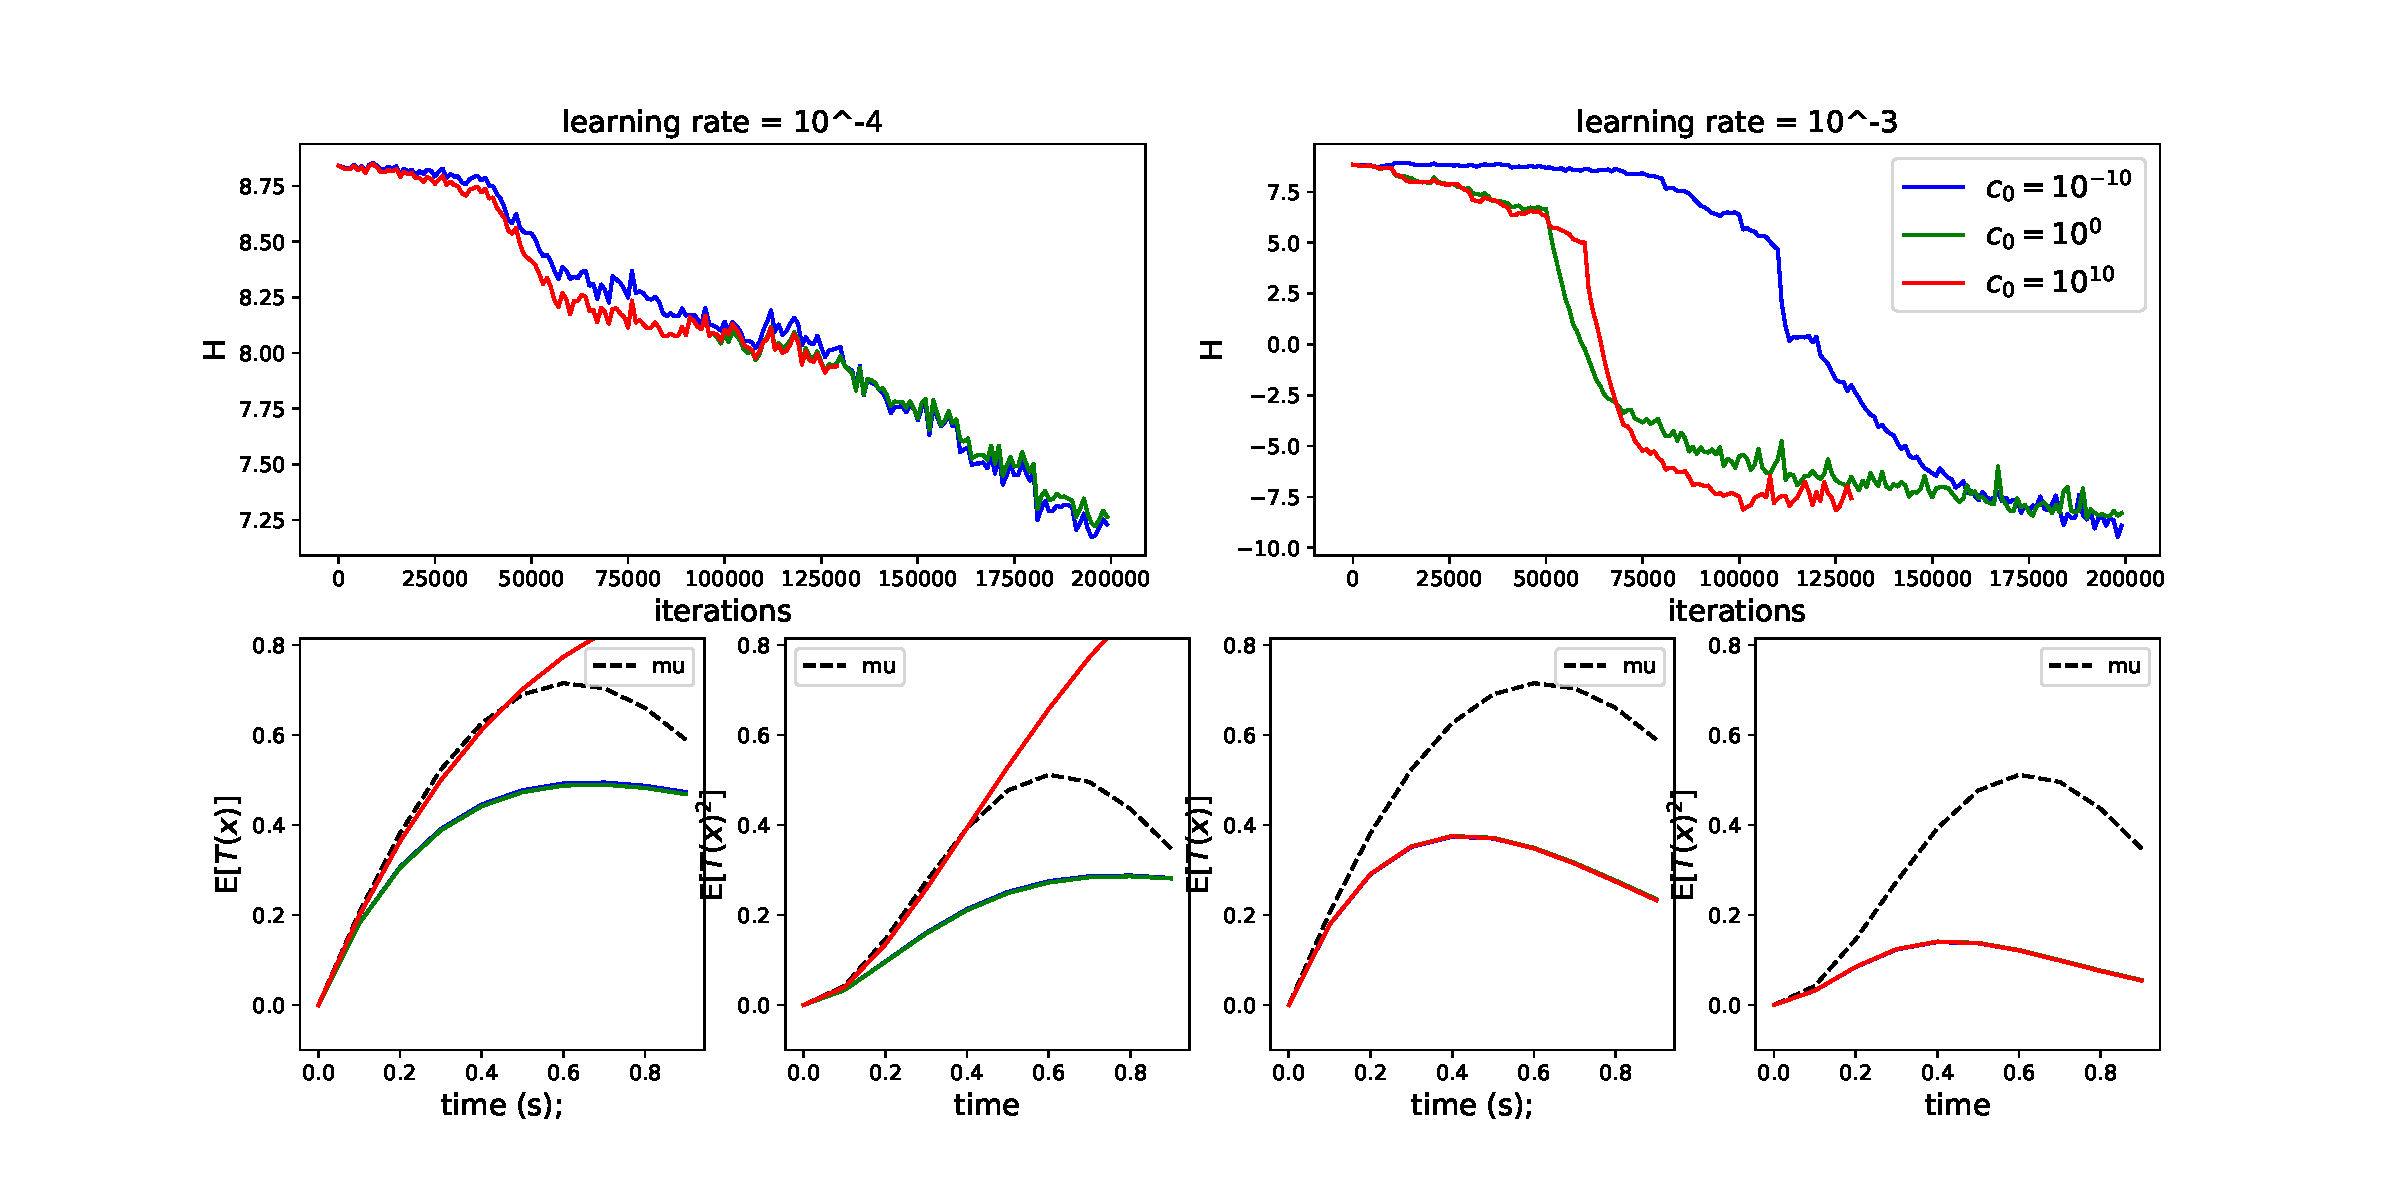
\includegraphics[scale=.41]{images/DHO_5P_T=10.pdf} \\
\end{center}

\begin{center}
\textbf{DHO with T = 10, 10 planar flows}
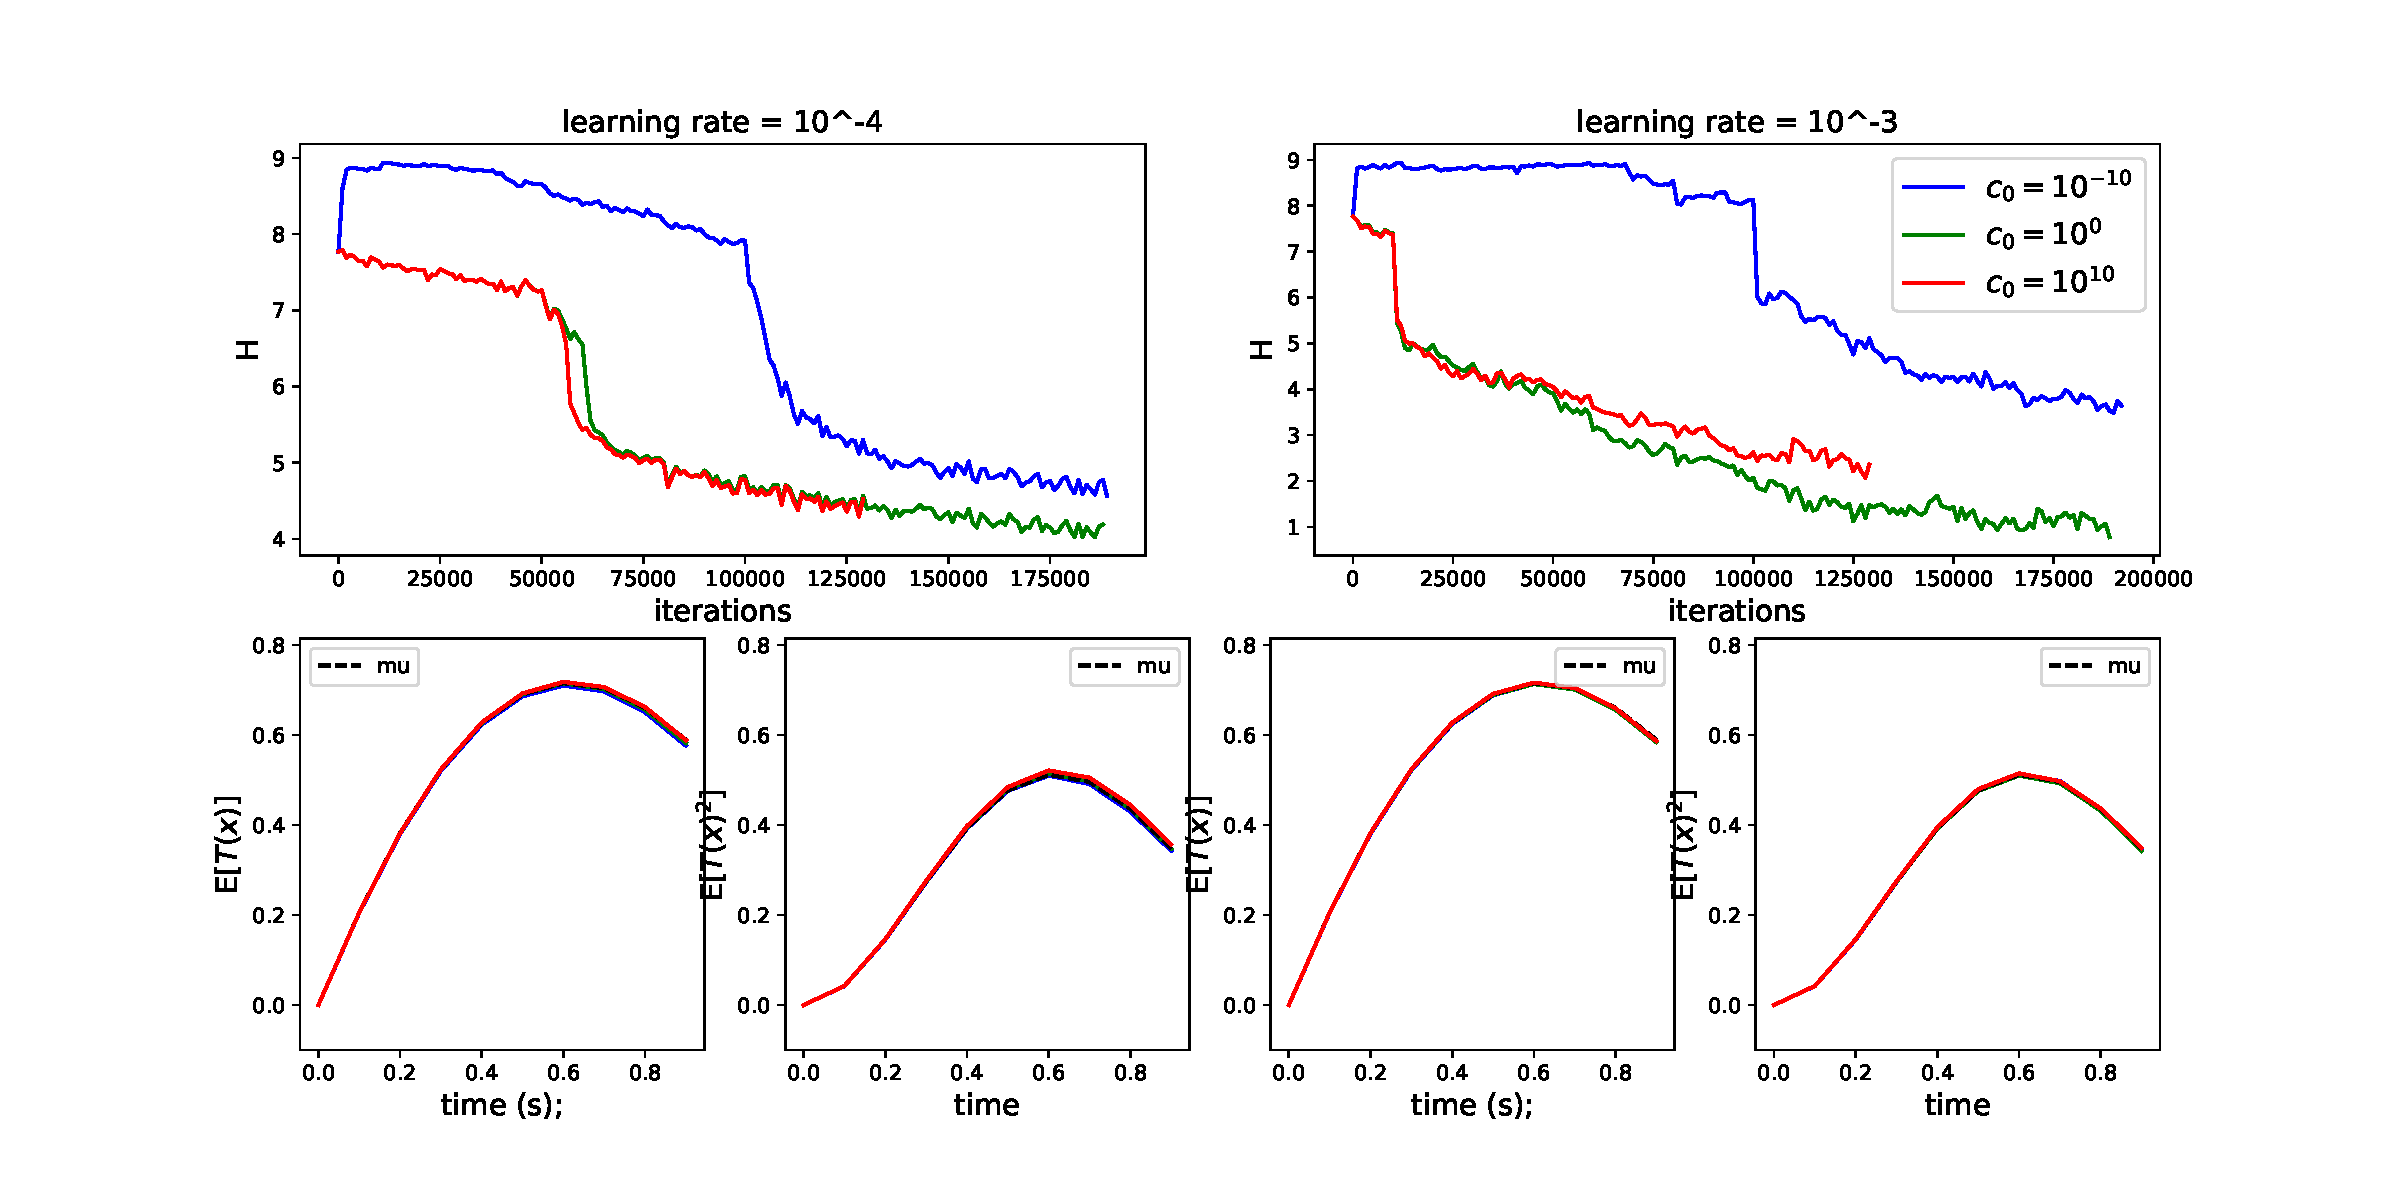
\includegraphics[scale=.41]{images/DHO_10P_T=10.pdf} \\
\end{center}
\clearpage

\begin{center}
\textbf{DHO with T = 30, 5 planar flows}
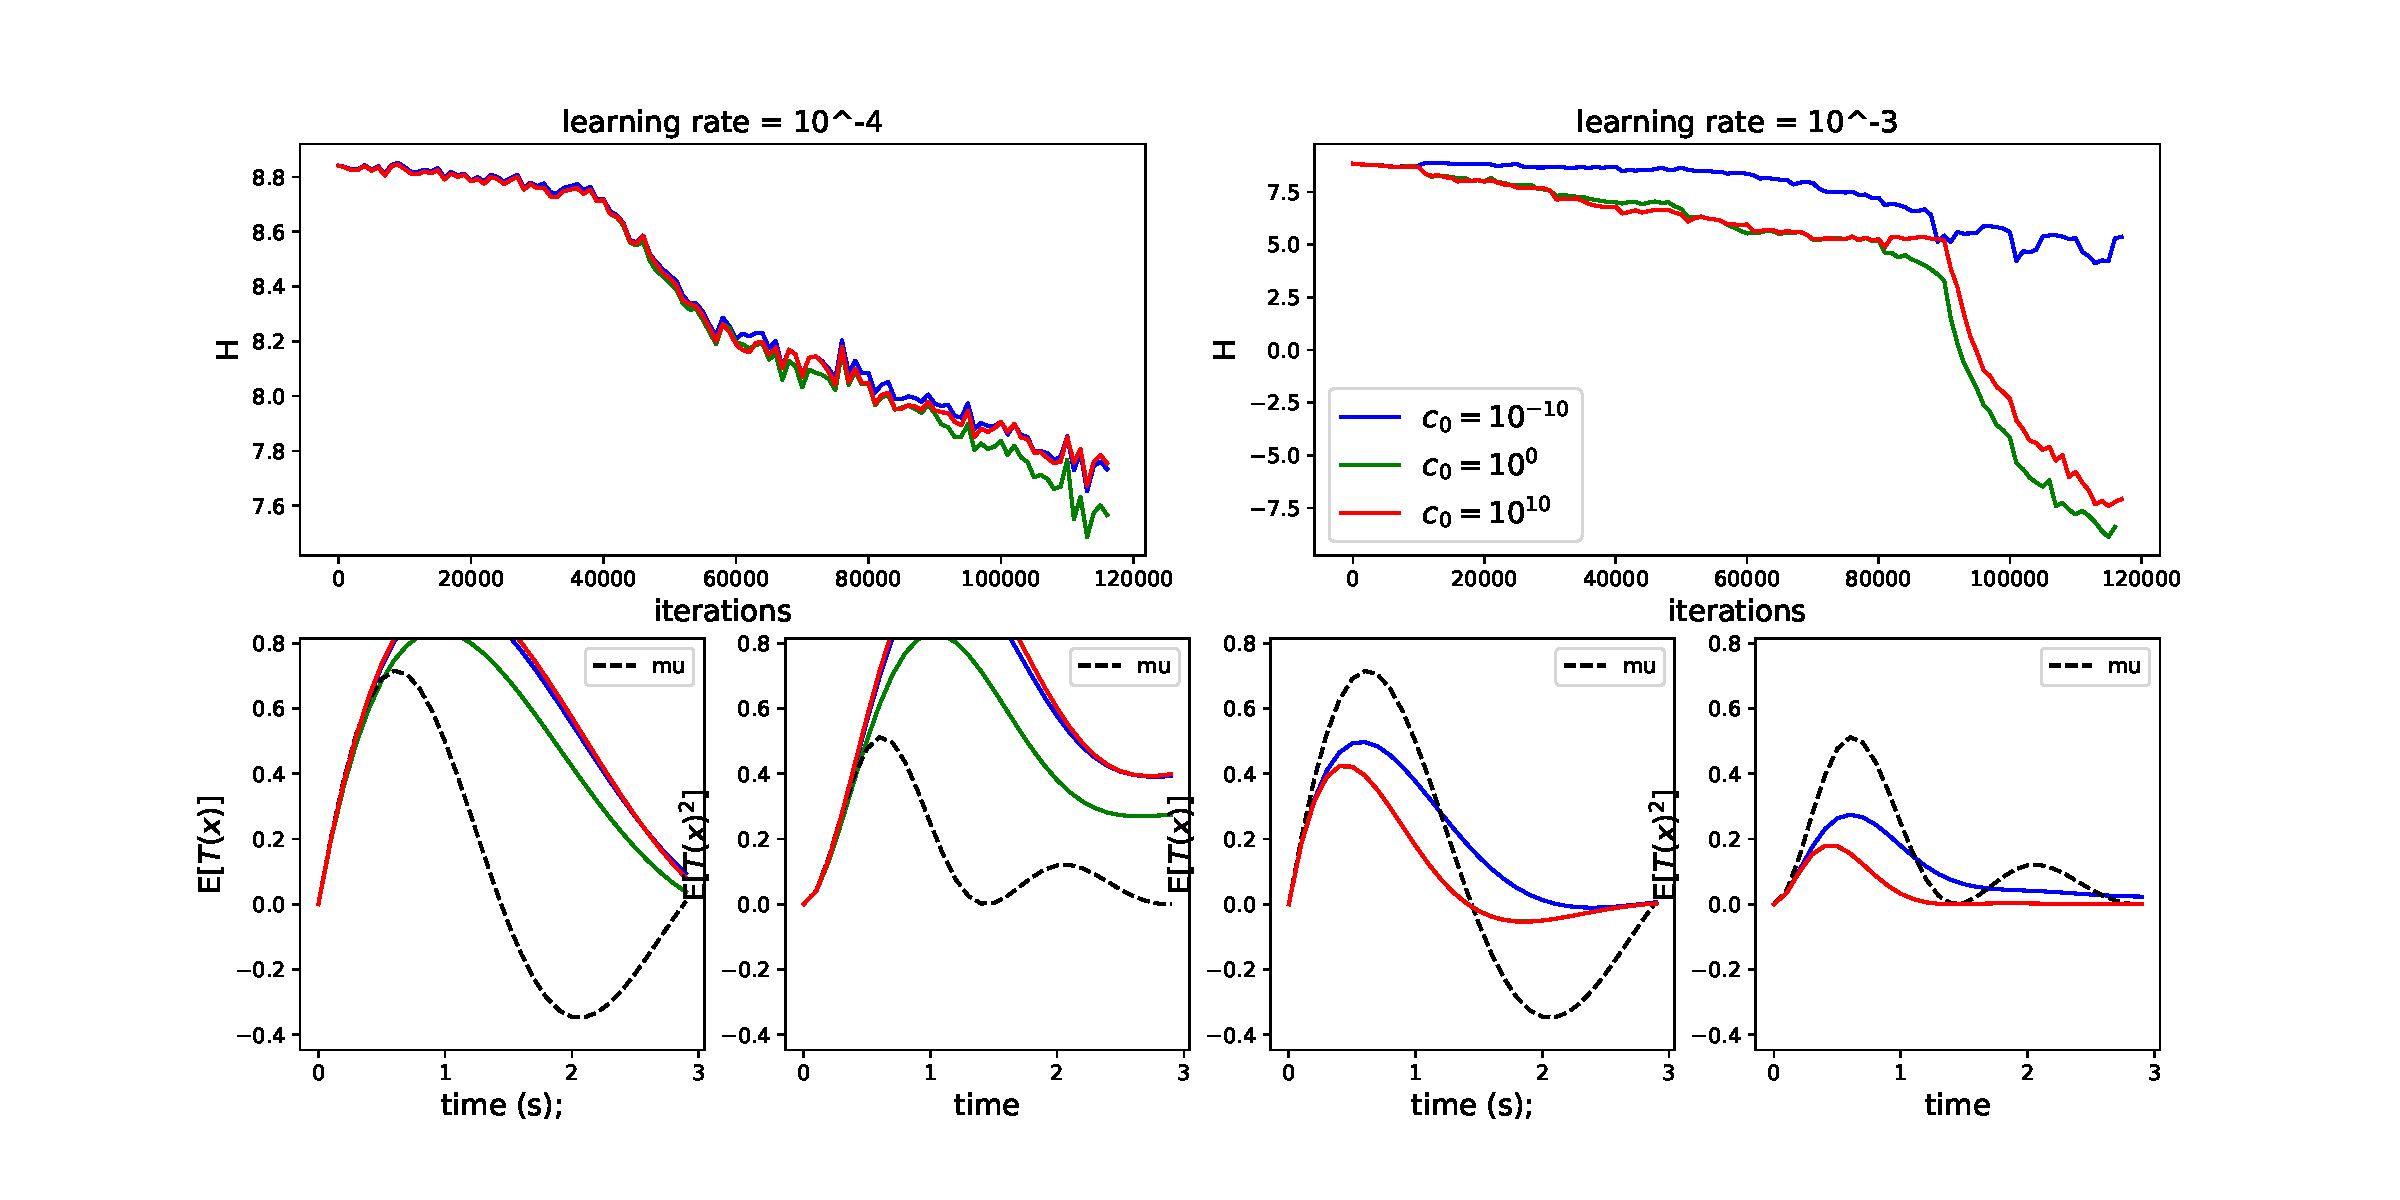
\includegraphics[scale=.41]{images/DHO_5P_T=30.pdf} \\
\end{center}

\begin{center}
\textbf{DHO with T = 30, 10 planar flows}
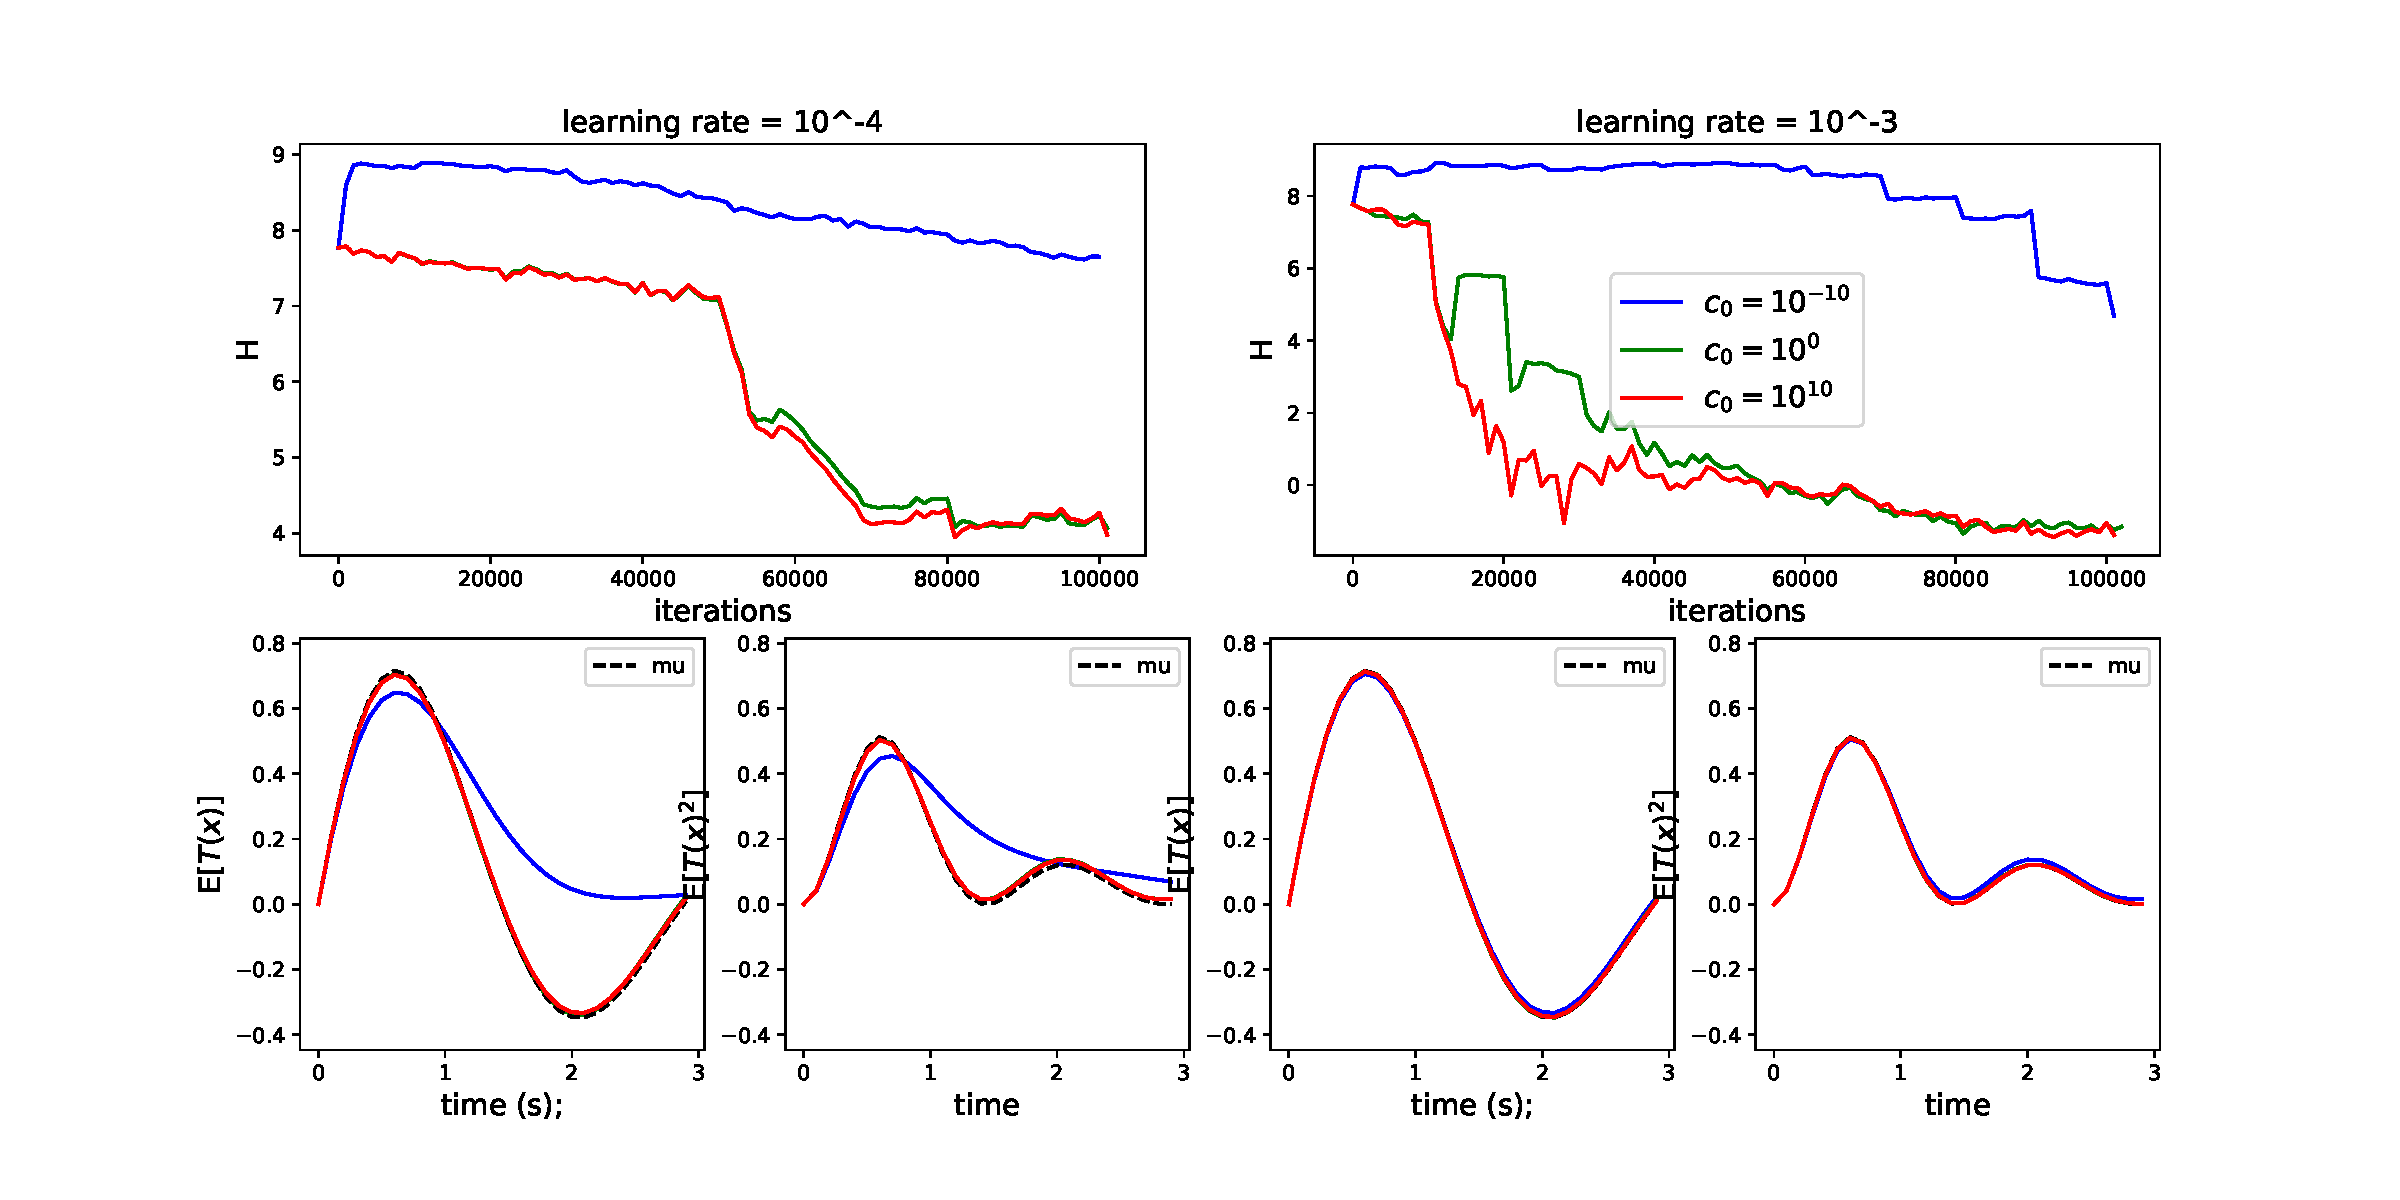
\includegraphics[scale=.41]{images/DHO_10P_T=30.pdf} \\
\end{center}
\clearpage

\begin{center}
\textbf{DHO with 10 planar flows $T=30$, $lr=10^{-3}$, $c_0=0$}
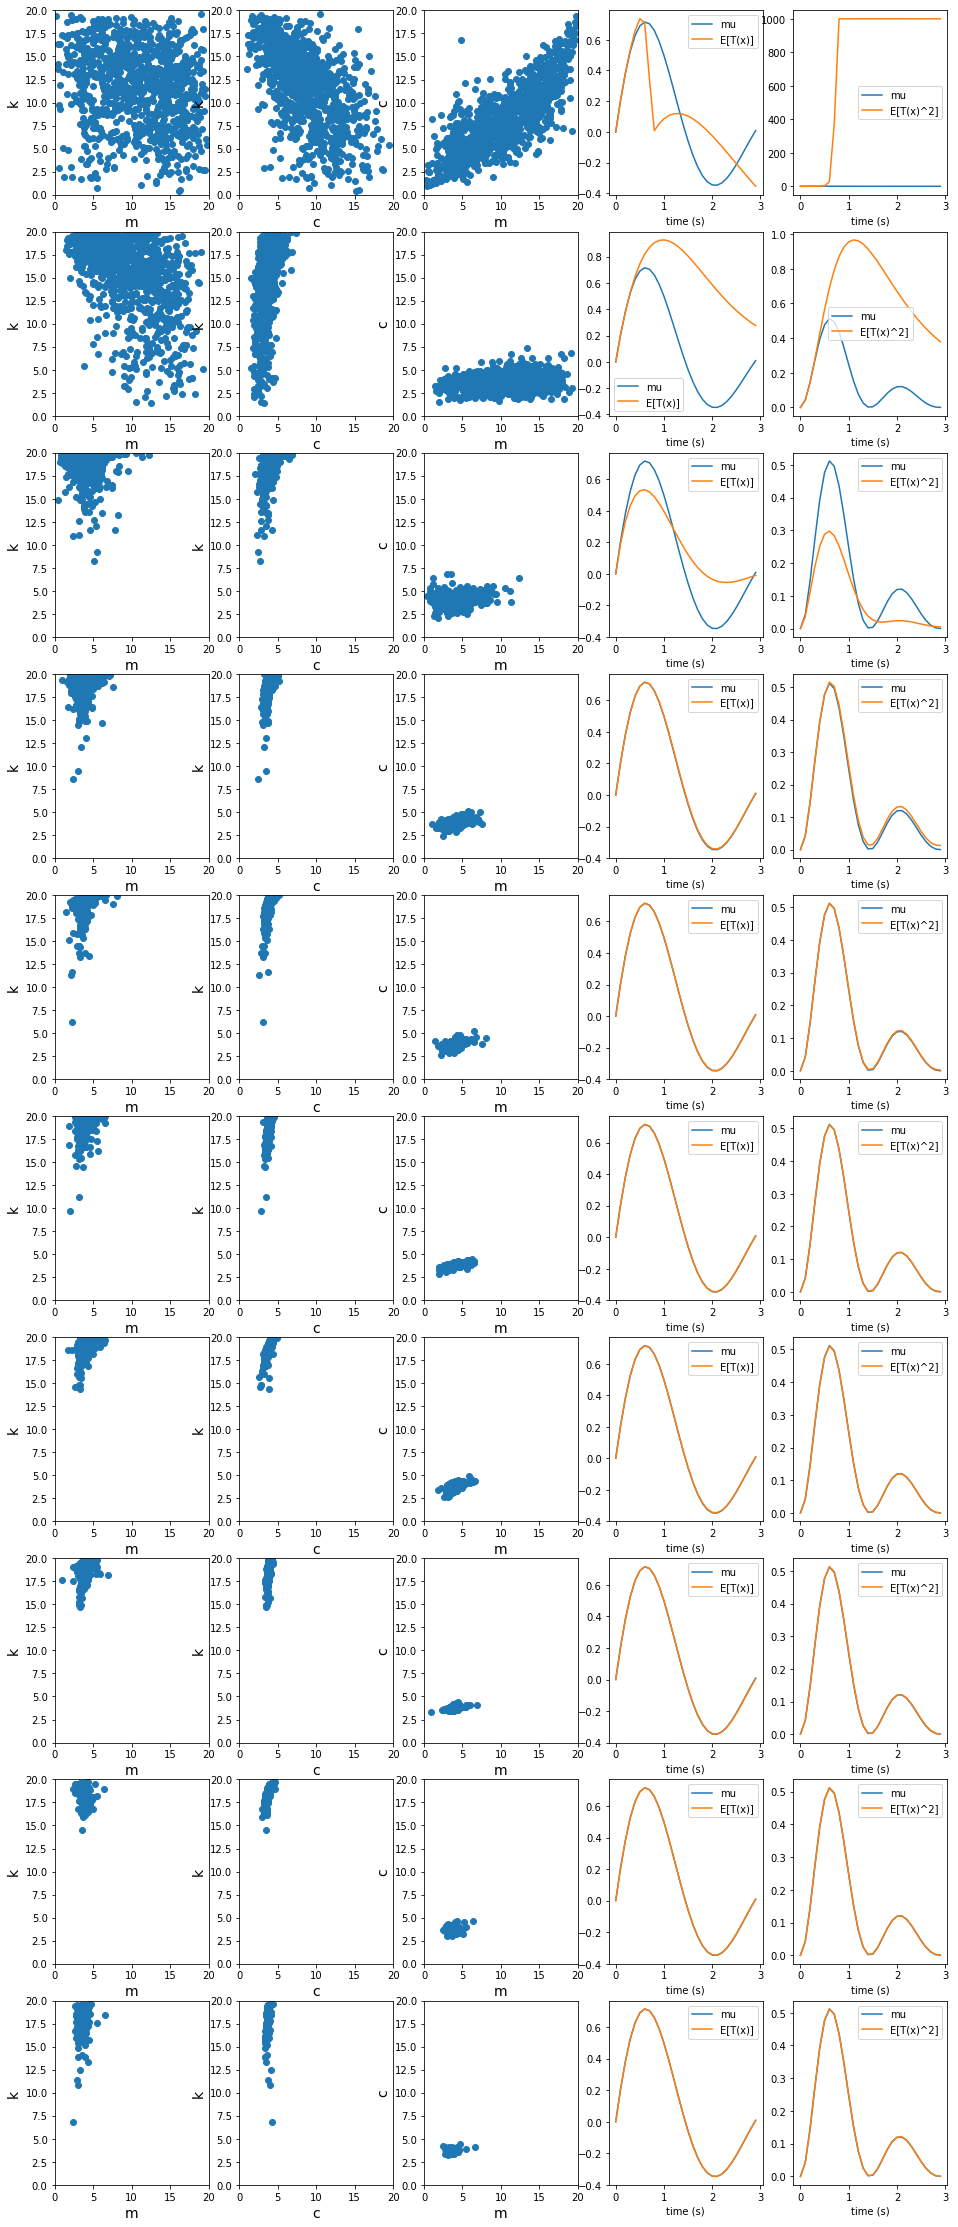
\includegraphics[scale=.25]{images/DHO_dist_10P_c=0_lr=-3_T=30.png} \\
\end{center}


\end{document}

